% 6.7 -- converted from manuscript.md lines 494-595 (source of truth).
\subsection{Type-D extension: preregistered C1-paired confirmation and C2-unpaired detection in Schwarzschild}\label{sec:schwarzschild}

The paired half of the capstone design transfers to the Schwarzschild
exterior on a measure identity: in Schwarzschild coordinates the volume
element is $\sqrt{-g} = r^2 \sin\theta$---independent of the mass and equal
to the flat spherical element---so one sprinkle of a coordinate patch serves
both geometries, exactly as $\det g = -1$ served the plane wave. What the
identity controls is the sampling measure; individual diamond volumes differ
under the two causal structures, and that difference is part of the signal
(the \sref{sec:pureweyl} distinction, unchanged). The frozen patch is the S1
solver domain ($M = 1$, exterior shell $r \in [10, 20]$, polar cap,
coordinate-time extent 40), with $N \sim \mathrm{Poisson}(300)$ events per
reading and the S1 predicate at tolerance $1\times10^{-8}$ with escalation
to $1\times10^{-10}$.

An exploration stage (S3, seed-ledger disciplined, preserved with its raw
per-reading arrays) measured the paired shift and sized a preregistered
confirmation (S4). The frozen rule
(\artifact{docs/\allowbreak{}prereg/\allowbreak{}p14\_\allowbreak{}s4\_\allowbreak{}schwarzschild\_\allowbreak{}c1.md}) fixes two gates
evaluated on identified intervals with strict comparisons: a primary
detection gate (identified CI95 above the frozen threshold
$\varepsilon_{\mathrm{det}} = 0.0036$, about 10\% of the exploration anchor,
in the frozen negative direction) and a secondary replication gate (the
independent two-sample Welch CI95 of the S4$-$S3 difference inside
$\pm\varepsilon_{\mathrm{rep}} = \pm 0.0012$, one exploration reading-SD); a
verified inclusion makes the joint verdict numerically equivalent to the
replication gate at these margins. Branch powers were certified before the
freeze by resampling both blocks from a conservatively scaled empirical
distribution (20000/20000 on every branch, exact Clopper--Pearson 95\% lower
bound 0.9998), with a constructed negative-control battery proving each gate
can fail. The campaign ran once, from the exact freeze checkout, with an
8-file content-addressed manifest verified at entry and at exit; the frozen
gates and results are in \tref{tab:s4}.

\begin{table}[t]
\caption{S4 frozen gates and results.}
\label{tab:s4}
\centering
\footnotesize
\begin{tabular}{@{}>{\raggedright\arraybackslash}p{6.5pc}>{\raggedright\arraybackslash}p{10pc}>{\raggedright\arraybackslash}p{11pc}>{\raggedright\arraybackslash}p{5.5pc}@{}}
\toprule
Gate & Frozen condition & Result & Verdict \\
\midrule
A: C1 detection (primary) & identified CI95 top $< -0.0036$ & CI95 $[-0.036211,\, -0.035953]$ & pass ($10\times$ margin) \\
B: replication (secondary) & Welch CI95 of S4$-$S3 inside $\pm 0.0012$ & $[-0.000183,\, +0.000194]$ & REPLICATED \\
\bottomrule
\end{tabular}
\end{table}

Stage verdict: CONFIRMED. The census recorded zero ambiguous pairs and one
escalated pair, resolved at the tighter tolerance. The frozen sentences are
recorded in Korean in the artifact
(\artifact{docs/\allowbreak{}prereg/\allowbreak{}p14\_\allowbreak{}s4\_\allowbreak{}results.json}) and quoted verbatim
(byte-exact with the artifact), each followed by a non-frozen English
translation:
``동결된 Schwarzschild 좌표·도메인(M=1, r∈[10,20], 극관각 캡 1.0, T=40)의 공통 측도 위에서, paired 앙상블 평균 이동의 identified CI95가 동결 방향으로 검출문턱 ε\_det = 0.0036을 초과했다 — 유한밀도 인과 census가 type D 진공 곡률의 빛원뿔 변형을 C1-급으로 검출했다(프로그램 내부 진술).''
(\textit{on the frozen Schwarzschild coordinates and domain, the paired
ensemble mean shift exceeds the frozen detection threshold in the frozen
direction---a finite-density causal census detects the light-cone
deformation of type-D vacuum curvature at C1 grade; a program-internal
statement});
``S4 블록과 S3 탐색 블록의 독립 두-표본 차이의 identified Welch CI95가 ±ε\_rep = ±0.0012 안에 들어, 탐색 효과가 정량적으로 재현됐다.''
(\textit{the independent two-sample difference between the S4 and S3 blocks
lies inside the replication band: the exploration effect is quantitatively
reproduced}).

A second, separate preregistered stage (S5) carries the single-poset claim
class. Guided by a committed stored-data feasibility audit
(\artifact{docs/\allowbreak{}prereg/\allowbreak{}p14\_\allowbreak{}c2\_\allowbreak{}feasibility\_\allowbreak{}audit.json}, exploratory, zero
additional solver calls, conservatively anchored), its rule
(\artifact{docs/\allowbreak{}prereg/\allowbreak{}p14\_\allowbreak{}s5\_\allowbreak{}schwarzschild\_\allowbreak{}c2.md}) declares---before
sizing and independently of the confirmation data---AUC 0.60 as the minimum
practically useful single-poset discrimination. Two \emph{independent} arms
(fresh Schwarzschild and fresh flat sprinkles; 300 readings each by a
pre-declared minimum-$n$ rule with directly certified branch powers) score
each reading by its global relation fraction; the primary gate is an
unclipped DeLong~\cite{delong1988} AUC CI95 with a four-way outcome (detected /
equivalent-at-margin / direction-reversed / inconclusive, strict
comparisons, identified-agreement across the curved bound series), and a
secondary out-of-sample balanced-accuracy gate uses a deterministic
Clopper--Pearson--Bonferroni interval with a train-half-only threshold. The
campaign ran once from its own exact freeze checkout; the frozen gates and
results are in \tref{tab:s5}.

\begin{table}[t]
\caption{S5 frozen gates and results.}
\label{tab:s5}
\centering
\footnotesize
\begin{tabular}{@{}>{\raggedright\arraybackslash}p{8.5pc}>{\raggedright\arraybackslash}p{7pc}>{\raggedright\arraybackslash}p{11.5pc}>{\raggedright\arraybackslash}p{5.7pc}@{}}
\toprule
Gate & Frozen condition & Result & Verdict \\
\midrule
Primary: AUC (DeLong) & CI95 lower $> 0.60$ & AUC 0.9734, CI95 $[0.9630,\, 0.9837]$ & \textbf{DETECTED} \\
Secondary: out-of-sample BA & joint CI95 lower $> 0.60$ & BA 0.9033, CI95 $[0.8356,\, 0.9500]$ & pass \\
\bottomrule
\end{tabular}
\end{table}

\begin{figure}[t]
\centering
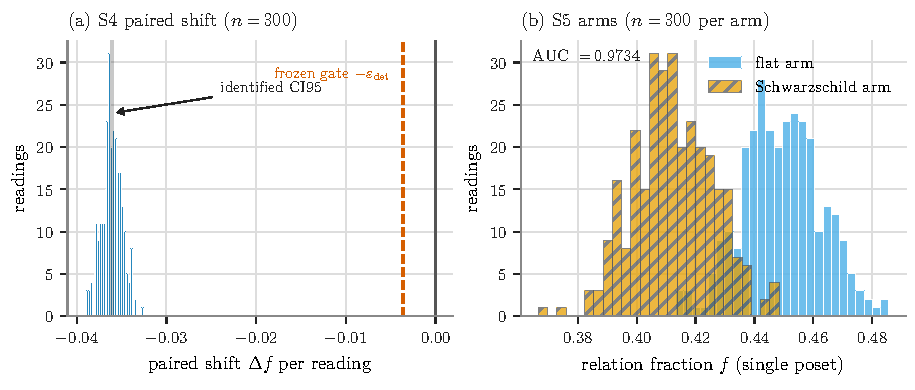
\includegraphics[width=0.95\textwidth]{figures/fig5_schwarzschild.pdf}
\caption{The Schwarzschild extension. (a)~The per-reading paired shift under
the frozen Schwarzschild domain: the identified CI95
$[-0.036211, -0.035953]$ lies an order of magnitude beyond the frozen
detection threshold $\varepsilon_{\mathrm{det}} = 0.0036$ (frozen negative
direction). (b)~The per-reading global relation fraction of the two
independent arms, discriminating with AUC 0.9734 (DeLong CI95
$[0.9630, 0.9837]$)---strong but, unlike the plane-wave C2, incomplete
separation. Drawn from the committed artifacts
(\artifact{docs/\allowbreak{}prereg/\allowbreak{}p14\_\allowbreak{}s4\_\allowbreak{}results.json},
\artifact{docs/\allowbreak{}prereg/\allowbreak{}p14\_\allowbreak{}s5\_\allowbreak{}results.json}); no value is typed in.}
\label{fig:schwarzschild}
\end{figure}

Zero ambiguous and zero escalated pairs; both identified bound series agree.
The frozen sentences are recorded in Korean in the artifact
(\artifact{docs/\allowbreak{}prereg/\allowbreak{}p14\_\allowbreak{}s5\_\allowbreak{}results.json}) and quoted verbatim
(byte-exact), each followed by a non-frozen English translation:
``동결된 Schwarzschild 도메인·밀도에서, 단일 causal set의 global relation fraction은 flat/Schwarzschild 앙상블을 우연 수준보다 판별하는 정보를 운반한다 (AUC CI95 하한 > 0.60, 프로그램 내부 진술).''
(\textit{on the frozen Schwarzschild domain and density, the global relation
fraction of a single causal set carries information that discriminates flat
from Schwarzschild ensembles above chance---AUC CI95 lower bound above 0.60;
a program-internal statement});
``out-of-sample balanced accuracy의 결합 95\% 하한이 0.60을 넘어, 학습-외 판별이 확인됐다 (secondary).''
(\textit{the joint 95\% lower bound of out-of-sample balanced accuracy
exceeds 0.60: out-of-training discrimination holds; a secondary verdict}).

What this extends, and at what grade: on the same frozen Schwarzschild
domain, the two claim classes of the plane-wave capstone are now each
supported by a \emph{separate} preregistered stage
(\fref{fig:schwarzschild})---the C1 paired claim CONFIRMED (S4), C2
single-poset discrimination DETECTED (S5). There was no joint primary
verdict, and the grades differ from the plane wave: its C2 separation was
complete, while the Schwarzschild discrimination is strong but imperfect
(AUC $\approx 0.973$; no completeness gate was preregistered); the secondary
BA verdict neither strengthens nor combines with the primary. The extension
establishes no mass-generality (a single frozen $M$) and uses no
diamond-volume oracle (margins operationally anchored or independently
declared)---the mass ladder and the certified-volume anchor belong to the
separate stage of \sref{sec:count}, which does not promote these two
verdicts. Execution provenance for both stages, including the
executed-freeze manifest snapshots---and the capstone's own freeze
ordering, mechanical gates, and commit-ancestry contract---is in
appendix~\ref{app:provenance}.
